\subsection{Activities}

%%%%%%%%%%%%%%%%%%%%%%%%%%%%%%%%%%%%%%%%%%%%%%%%%%%%%%%%%%%%%%%%%%%%%%

\subsubsection{Stereo vision depth detection}
\begin{itemize}
	\item Camera frames are read by the CPU.
	\item CPU writes the images to the GPU.
	\item Designed the rendering pipeline needed by our application.
	\item The pipeline generates the following framebuffers:
	\begin{itemize}
		\item \textbf{Encoding:} This is the same data than the original image, but using the RGBA channels to pack four GL\_LUMINANCE 	pixels into a GL\_RGBA pixel. See figure~\ref{fig_pixel_pack} for a graphical explanation.
		\item \textbf{Support window:} This puts in every pixel information about its surrounding pixels. The objective is to make the calculation of the disparity map computationally cheaper. See figure~\ref{fig_support_window} for a graphical explanation.
		\item \textbf{Disparity map:} This looks for the disparity where the similarity of the support windows is a minimum and generates a texture with this information.
	\end{itemize}
\end{itemize}

\begin{figure}[ht!]
\begin{center}
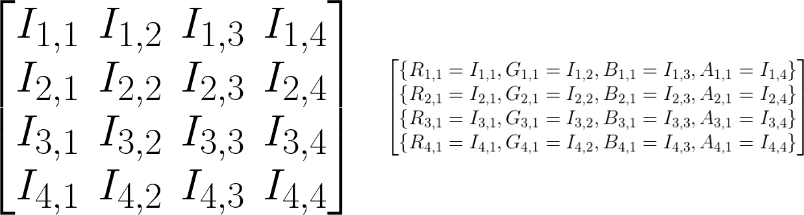
\includegraphics[height=0.22\textwidth]{fig/pixel_pack}\\
\caption{4x4 GL\_LUMINANCE texture (left) losslessly packed into a 4x1 GL\_RGBA texture (right).}
\label{fig_pixel_pack}
\end{center}
\end{figure}

\begin{figure}[ht!]
\begin{center}
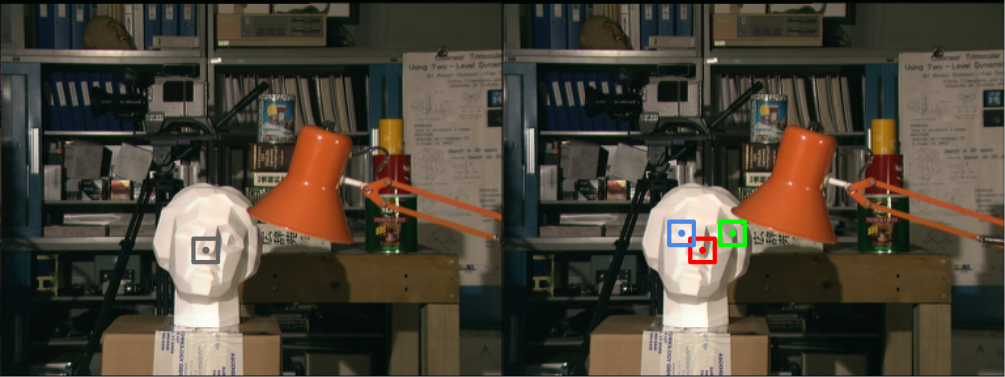
\includegraphics[height=0.40\textwidth]{fig/support_window}\\
\label{fig_support_window}
\caption{Support window to match (left) and the windows attempted/scanned on the other image (right).}
\end{center}
\end{figure}


%%%%%%%%%%%%%%%%%%%%%%%%%%%%%%%%%%%%%%%%%%%%%%%%%%%%%%%%%%%%%%%%%%%%%%

\subsubsection{Midterm presentation}
\begin{itemize}
	\item Did a presentation with the following information:
	\begin{itemize}
		\item Introduction.
		\item Challenges.
		\item Some theory.
		\item Tables and diagrams providing a picture of the work being done.
		\item Conclusions (so far).
	\end{itemize}
	\item The presentation can be found \href{https://docs.google.com/presentation/d/1_rqsAgTJxvEJvtRudIc00ItqAo_ZehuIC6Ru60WV8h8/edit?usp=sharing}{at this link}.
\end{itemize}

